\section{Architecture: Minimal Changes to the Vehicle}
\label{sec:architecture}

Minimal fleets only work if converting one car is cheap and simple. So we state the architecture as a bill of changes: what we add to an existing car, and what we leave alone (Figure~\ref{fig:architecture}). We add four functions, sensing, an ego-centric digital twin, a learned advisory policy, and a safety and etiquette filter, plus a display; nothing else changes. There is no connection to the throttle, brakes, steering, or the CAN control plane. The OBD-II port, on every US car since 1996, is only read, to get the car's speed. No identity leaves the vehicle, and no server sits in the real-time loop. The kit installs like a dashcam.

\begin{figure}[t]
\centering
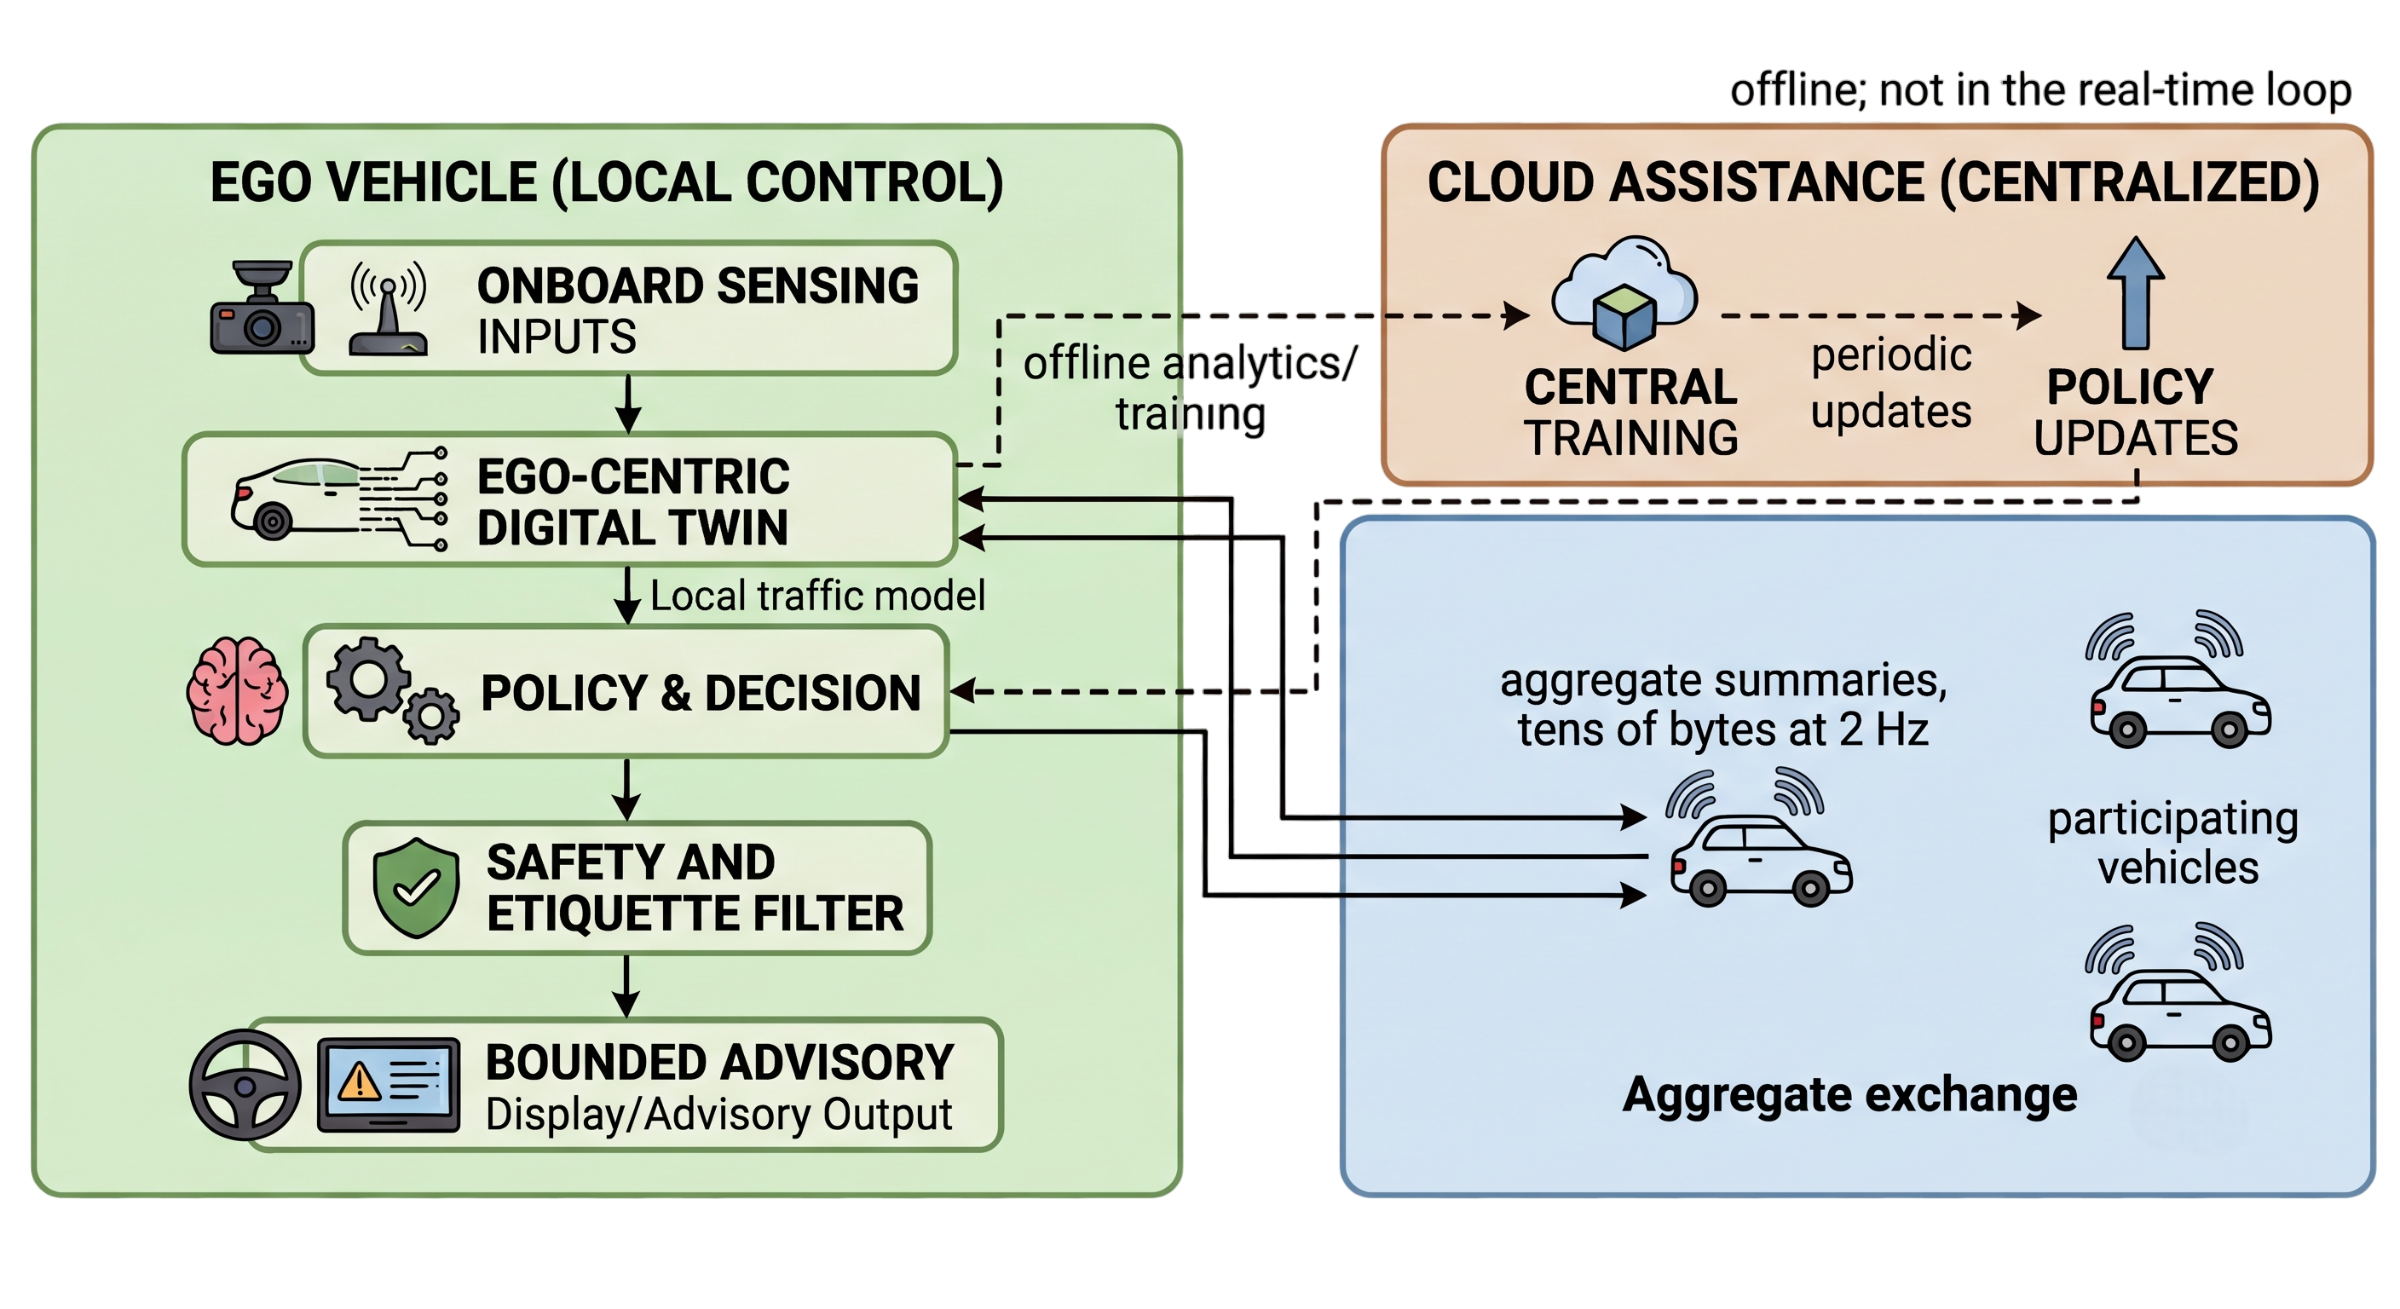
\includegraphics[width=\columnwidth,height=0.50\columnwidth,keepaspectratio]{images/system_architecture.png}
\caption{The self-regulating retrofit. Onboard sensing feeds an ego-centric digital twin; a learned policy proposes a coarse action; a safety and etiquette filter bounds what is shown as an advisory. Peer vehicles broadcast small aggregate summaries that widen the twin's view; the cloud only trains and ships model updates offline, never in the real-time loop.}
\Description{Block diagram of the on-vehicle pipeline from sensing through digital twin, policy, and safety filter to a bounded advisory, with peer broadcast summaries entering the twin and an offline cloud path for training and model updates.}
\label{fig:architecture}
\end{figure}
% TODO: replace images/system_architecture.pdf with the final diagram export; caption is written for the corrected version (advisory terminus, no V2V hub, dashed offline cloud edges).

\noindent\textbf{Sensing and fusion.}
Each vehicle estimates its immediate scene from its own sensors: ego speed, acceleration, lane, headway, leader and follower gaps, relative speeds, local density, a queue estimate, and distance to a merge. Aggregate summaries, when heard, add peer-derived state over a bounded radius. The combined observation is deliberately not a global state but a local one, with a few hints about what lies beyond the camera. The deployment stack mirrors the simulator's observation contract instead of inventing a separate API: in our prototype a 39-field vector copied unchanged from the training code and checked bit for bit by tests. Every field is logged with its provenance (measured, derived, fallback-neutral, static, or sim-parity). Leader gap and closing speed come from forward tracks, density from forward counts, rear-lane fields from neutral fallbacks until a rear camera is added, and nearby-vehicle fields from peer summaries when enabled. This record of where each value came from tells the policy and the safety layer how much to trust the observation.

\noindent\textbf{The ego-centric digital twin.}
At runtime, each vehicle keeps a small, continuously updated model of its local road state: the ego vehicle, nearby vehicles, lane structure, merge pressure, and short-horizon congestion risk. This is the digital twin. It is a compact tracker, not a city-scale simulator running in the car, and its job is to widen what the car can act on. It lets the controller reason about density and downstream pressure it can only partly see, and it lets the safety layer test an advisory against a short-horizon prediction before it is shown. The twin also records when each aggregate was last refreshed and where it came from, so the policy can tell ``I see no cooperating vehicles'' apart from ``the radio is stale'', and the safety layer can reject advice built on shaky state.

\noindent\textbf{Centralized training, decentralized execution.}
Training is centralized; execution is not. During training, a simulator or a logged fleet can expose global state and what-if rollouts; at run time, the policy sees only onboard sensing and local aggregate fields, so nothing central is needed to drive. This division of labor, learning and coordination in the cloud, sensing and control at the edge, is the system's central placement decision, and the bridge from the centralized predecessor~\cite{self_regulating_cars} to a vehicle-native one. Because a deployed policy will meet merge geometries, demand patterns, and compliance levels it never trained on, we view model-based reinforcement learning, learning a model of road dynamics and adapting the policy inside it, as the most promising route to handling new road layouts without huge amounts of new driving data~\cite{sutton1991dyna,janner2019trust,hafner2020dream}.

\noindent\textbf{Advisory control.}
The outputs stay conservative: a speed bin ('slow', 'nominal', 'fast'), a headway bin, a cautious lane preference, and a merge mode, never raw throttle, braking, or aggressive lane-change commands. Prior work on self-regulating cars shows that coarse bins like these are enough for a learned policy to improve flow and reduce hard braking~\cite{self_regulating_cars}; coarse bins are also what a human driver can follow. With a human in the loop, the output is a bounded advisory in the spirit of prior advisory-autonomy work~\cite{Yan_2023,cho2023temporal,fridman2018human}; in an automated vehicle, it can feed the existing longitudinal controller. Either way, the self-regulation layer nudges the car toward network-friendly behavior without claiming authority over it.

\noindent\textbf{Safety and etiquette filter.}
Every advisory passes through a local filter before it is shown or executed. The filter enforces posted speed limits, acceleration and braking bounds, minimum front and rear gaps, target-lane time-to-collision margins, lane-change dwell and rate caps, and a limit on how much braking an advisory may force on followers. It also blocks low-speed behavior on an open road and synchronized all-lane slowdowns unless downstream congestion justifies them. Every blocked or changed action is reported under a stable label: safety-masked, etiquette block, follower-disruption block, or external override. This layer is what makes it safe to pursue a network goal in mixed human traffic; it also means the action to train on and measure is the one the car actually took, not the raw proposal.

\noindent\textbf{Degraded operation.}
The edge design follows one rule: stale data is worse than missing data. If GPS goes stale, the observation builder holds the last valid speed for a short window instead of reporting a stop, and if no peers are heard, cooperation fields revert to explicit neutral values, not silent zeros. These modes turn common in-car failures into explicit states instead of hidden dependencies.

\noindent\textbf{Deployment tiers.}
The same architecture can be built three ways, and the tiers differ only in which observation fields are truly measured and which stay at neutral defaults, a difference the provenance record makes visible to the policy. \emph{Tier 0} is an app: a phone already has the GPS, inertial sensing, and compute for the observation builder and a two-layer policy, camera optional. The advisory rail for this tier runs at scale today: mobile telematics platforms such as CMT and Samsara deliver real-time driving feedback through phone apps and lightweight tags, CMT alone measuring tens of millions of drivers daily~\cite{cmt2025,samsara2025}. The predecessor argued this makes app-level integration a credible path to system-level coordination without infrastructure changes~\cite{self_regulating_cars}; our design inherits that path and removes its runtime dependency, shrinking the cloud to training, updates, and offline analytics. \emph{Tier 1} is a retrofit kit, the prototype of Section~\ref{sec:eval}: a windshield camera, a USB GPS receiver, an optional OBD-II dongle as the preferred speed source, an embedded board that retails for roughly \$250~\cite{nvidia2023jetson}, and any display. \emph{Tier 2} is native: a vehicle with automated longitudinal control takes the filtered advisory as a set-point. Deployment is minimal and incremental by construction: a fleet can mix tiers, add one car at a time, and never touch the road, making the 25-vehicle deployment of Section~\ref{sec:vision} an operational decision, not a hardware program.
